

\documentclass[a4paper,12 pt]{article}
\usepackage{graphicx}
\usepackage{caption}
\usepackage{refstyle}
\usepackage{wrapfig}
\usepackage{subcaption}
\usepackage{geometry}
 \geometry{
 a4paper,
 total={210mm,297mm},
 left=25mm,
 right=25mm,
 top=25mm,
 bottom=25mm,
 }

\title {Project Report \\ Sensor Module Interfacing \\[10pt] Task: Interfacing Gyroscope with ATmega2560 in Firebird V Robot \\[25pt] Team members }
\author {Chayatan \and Mukilan A \and Shantanu}

\begin{document}
\maketitle
\begin{center}
\begin{large}
Under the guidance of\\
\textbf{Prof. Kavi Arya\\and\\Parin Chedda}\\
\vspace{0.5in}
\end{large}
\end{center}
\begin{center}

\includegraphics[scale=0.32]{iitb.png}
\end{center}
\begin{center}
\begin{large}
Embedded and Real-Time Systems Laboratory \\
Department of Computer Science and Engineering \\
Indian Institute of Technology \\
Bombay \\
\end{large}
\end{center}

\newpage
\tableofcontents
\newpage
%----------------------------------------------------------------------------------------------------------------
\begin{abstract}The project aims at interfacing a Gyroscope with Fire Bird V educational robot. This additional module can be used for measuring or maintaining the orientation, based on the principles of angular momentum. In this paper we will see about the basic L3G4200D Gyroscope module interfacing with Atmega 2560 in Fire Bird V robot. This will include the working principle, basic interfacing circuit, programming and applications of the Gyroscope.
\end{abstract}
%----------------------------------------------------------------------------------------------------------------
\section{Introduction}
\begin{wrapfigure}{r}{0.4\textwidth}
  \begin{center}
\vspace{-10mm}
    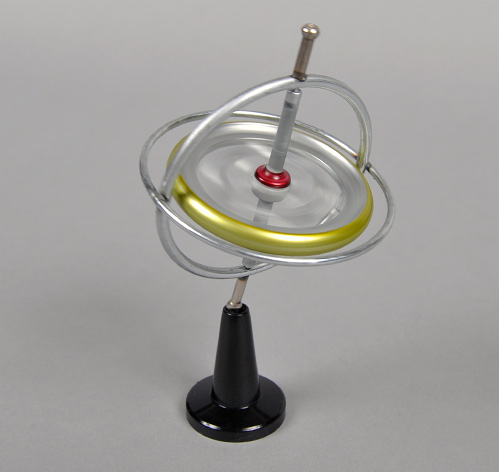
\includegraphics[scale=0.2]{Gyr0.jpg}
  \end{center}
  \caption{A Gyroscope}
\end{wrapfigure}

\ \ The root word in Gyroscope is derived from a Latin word ‘guros’ meaning ring. The basic model of a Gyroscope is a device that consists of a disc or a wheel that is spun rapidly around an axis, such that its orientation is independent of the tilting of the mounting. Hence, they are used in providing stability or in maintaining a reference direction in navigation systems, automatic pilots, and stabilizers.

In this document, we are going to discuss the Gyroscope sensor L3G4200D, and understand its interfacing with the FireBird V Robot.
%----------------------------------------------------------------------------------------------------------------
\section{Specifications of L3G4200D Gyroscope: }
\begin{itemize}
\item Onboard 3.3V Low Drop voltage regulator with input range of 3.6V to 6V.
\item Dimensions: 0.9”(L) X 0.5”(W)
\item 2 x Mounting holes
\item I2C/SPI digital output interface
\item Three selectable full scales (250/500/2000dps)
\item Sensitivity: 
\begin{itemize}
\item 250 dps : 8.75 mdps/digit 
\item 500 dps : 17.50 mdps/digit
\item 2000 dps : 70 mdps/digit
\end{itemize}

\item 16 bit data output
\item Embedded temperature sensor with 8-bit temperature data output
\item Integrated low- and high-pass filters with user selectable bandwidth
\item Embedded power-down and sleep mode
\item Extended operating temperature range (-40 °C to +85 °C)
\end{itemize}
%----------------------------------------------------------------------------------------------------------------
\pagebreak

\section{Pin Connections of L3G4200D:}
\subsection{Pin Diagram}
\begin{figure}[!h]
\begin{center}
 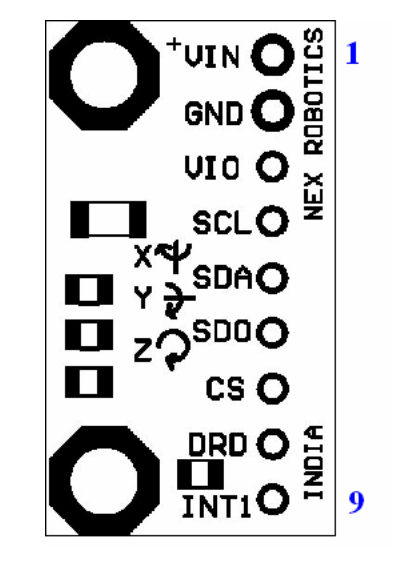
\includegraphics[scale=0.8]{gyr3.png}
\end{center}
\caption{Pin Diagram}
\label{fig:1}
\end{figure}
\newpage
\subsection{Useful Pins in the L3G4200D Gyroscope and its Connections with the Firebird V Robot}

\begin{figure}[!h]
\begin{center}
 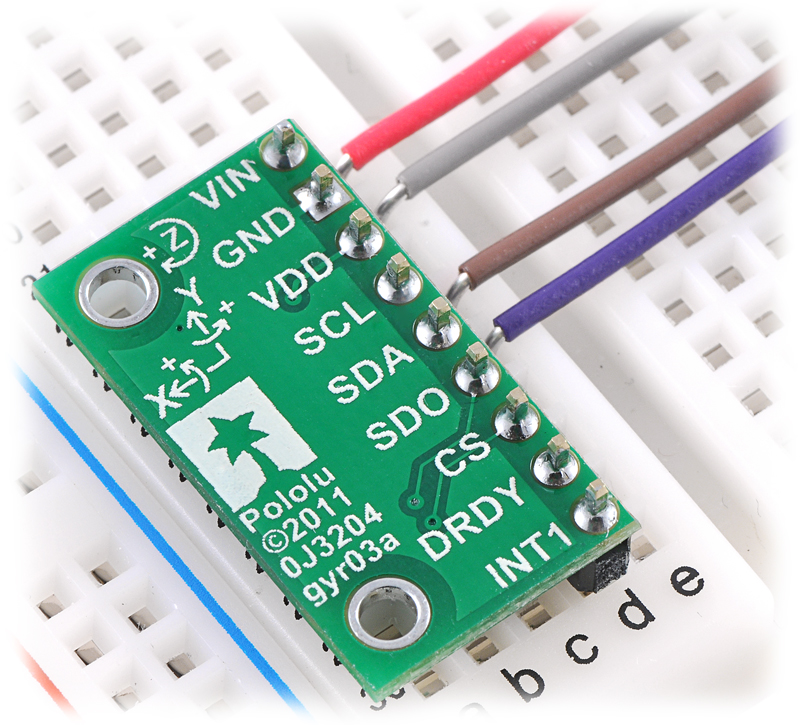
\includegraphics[scale=0.30]{gyr2.jpg}
\end{center}
\caption{Useful Pins in the L3G4200D Gyroscope}
\label{fig:1}
\end{figure}
%---------------------------------------------------------------------------------
\begin{figure}[!h]
\begin{center}
 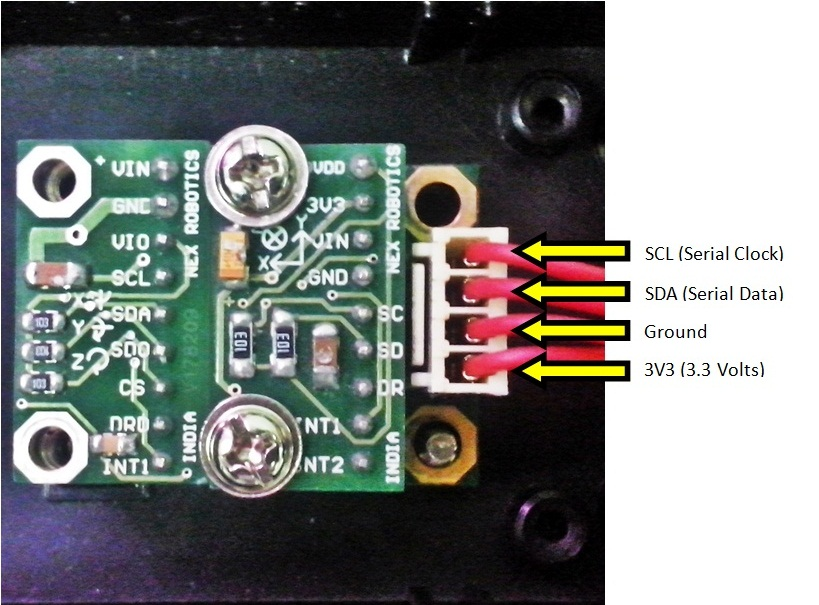
\includegraphics[scale=0.60]{gyr7.jpg}
\end{center}
\caption{Useful Pins in the L3G4200D Gyroscope}
\label{fig:1}
\end{figure}
%---------------------------------------------------------------------------------
\vspace{-10mm}
\begin{center}
\begin{table}[!h]
\hspace{-10mm}
\caption{}
\begin{tabular}{|c|c|}

\hline

$Pins of L3G4200D$&$Pins of Firebird V Robot $\\
Gyroscope Sensor$ $&$$\\
\hline
GND&Pin 23/24 (Ground) in Microcontroller Expansion Slot\\
\hline
Vin&3.3 Volts in Xbee Module in Firebird V\\
\hline
SDA&Pin 19 in Microcontroller Expansion Slot\\
\hline
SCL&Pin 20 in Microcontroller Expansion Slot\\


\hline
\end{tabular}
\label{table:t1}
\end{table}
\end{center}
\subsection{Communication between Firebird V and L3G4200D using I2C Protocol}
\textbf{I2C interface between L3G4200D and 3.3V microcontroller}

\begin{figure}[!h]
\begin{center}
 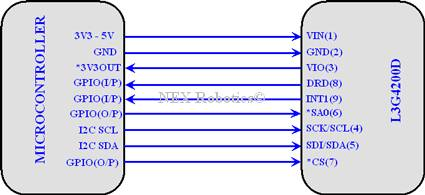
\includegraphics[]{gyr5.jpg}
\end{center}
\caption{I2C interface between L3G4200D and 3.3V microcontroller}
\label{fig:1}
\end{figure}

\newpage
\section{Procedure to interface IMU to FireBird V}
\subsection{Procedure to write data into a slave}
\begin{enumerate}

\item Send START condition to initiate the process.
\item Sending the start condition will generate an interrupt. Wait for TWINT flag to be set. 
\item Load SLA\_W into TWDR Register to switch to Master Write mode. The address is 0xD2 for gyroscope. 
\item Clear the TWINT flag to start transmission of slave address.
\item Wait for TWINT flag to be set which signifies that the slave address has been transmitted.
\item Send address of register byte that we want to access.
\item Clear the TWINT flag to start transmission of the register address.
\item Wait for TWINT flag set which means that an interrupt is generated for sending the register address.
\item Convert the character to equivalent BCD value and load into TWDR.
\item Clear the TWINT flag to start transmission of data byte.
\item Wait for the TWINT flag to be set.
\item Send STOP condition to terminate the data transfer.

\end{enumerate}


\subsection{Procedure to read data from a slave}
\begin{enumerate}
\item Send the START condition.
\item START condition sent will generate an interrupt. Wait for TWINT Flag set which means that the interrupt has occurred.
\item Load SLA\_W into TWDR Register to switch to Master Write mode.
\item Then clear the TWINT flag to start transmission of slave address.
\item Transmission of slave address will generate an interrupt. Wait for TWINT flag to be set. 
\item Send  the address of the register byte that we want to access.
\item Then clear the TWINT flag to start transmission of slave address.
\item Transmission of slave address will generate an interrupt. Wait for TWINT Flag to be set.
\item Send RESTART condition and start again to operate in Master Read mode.
\item RESTART condition sent will also generate an interrupt. So wait for TWINT Flag set which means that the interrupt has occured.
\item Load SLA\_R into TWDR Register to switch to Master Read mode. The address is D3 for Gyroscope.
\item Clear the TWINT flag to start the transmission of slave address.
\item Wait for TWINT flag to be set.
\item Clear the TWINT flag to read the addressed register.
\item Wait for the TWINT flag set.
\item Load the NO-ACK value to TWDR register.
\item Clear TWINT flag to start transmission of NO\_ACK signal.
\item Wait for TWINT flag to be set.
\item Now the value read can be used for any purpose.



\end{enumerate}

\textbf{Important Note:}
\begin{itemize}
\item SA0 pin is internally pulled up to VIO which sets LSB of I2C address as 1.
\item CS pin is internally pulled up to VIO which enables I2C mode.
\item 3V3OUT is capable of delivering 3.3V@ 40mAmps. It can be used set up pull ups for I/O pins related to L3G4200D. It should not be used for other purposes.
\end{itemize}
%\newpage
\section{Output of the Gyroscope L3G4200D}
\subsection{Output Displayed on LCD}
\begin{figure}[!h]
\begin{center}
 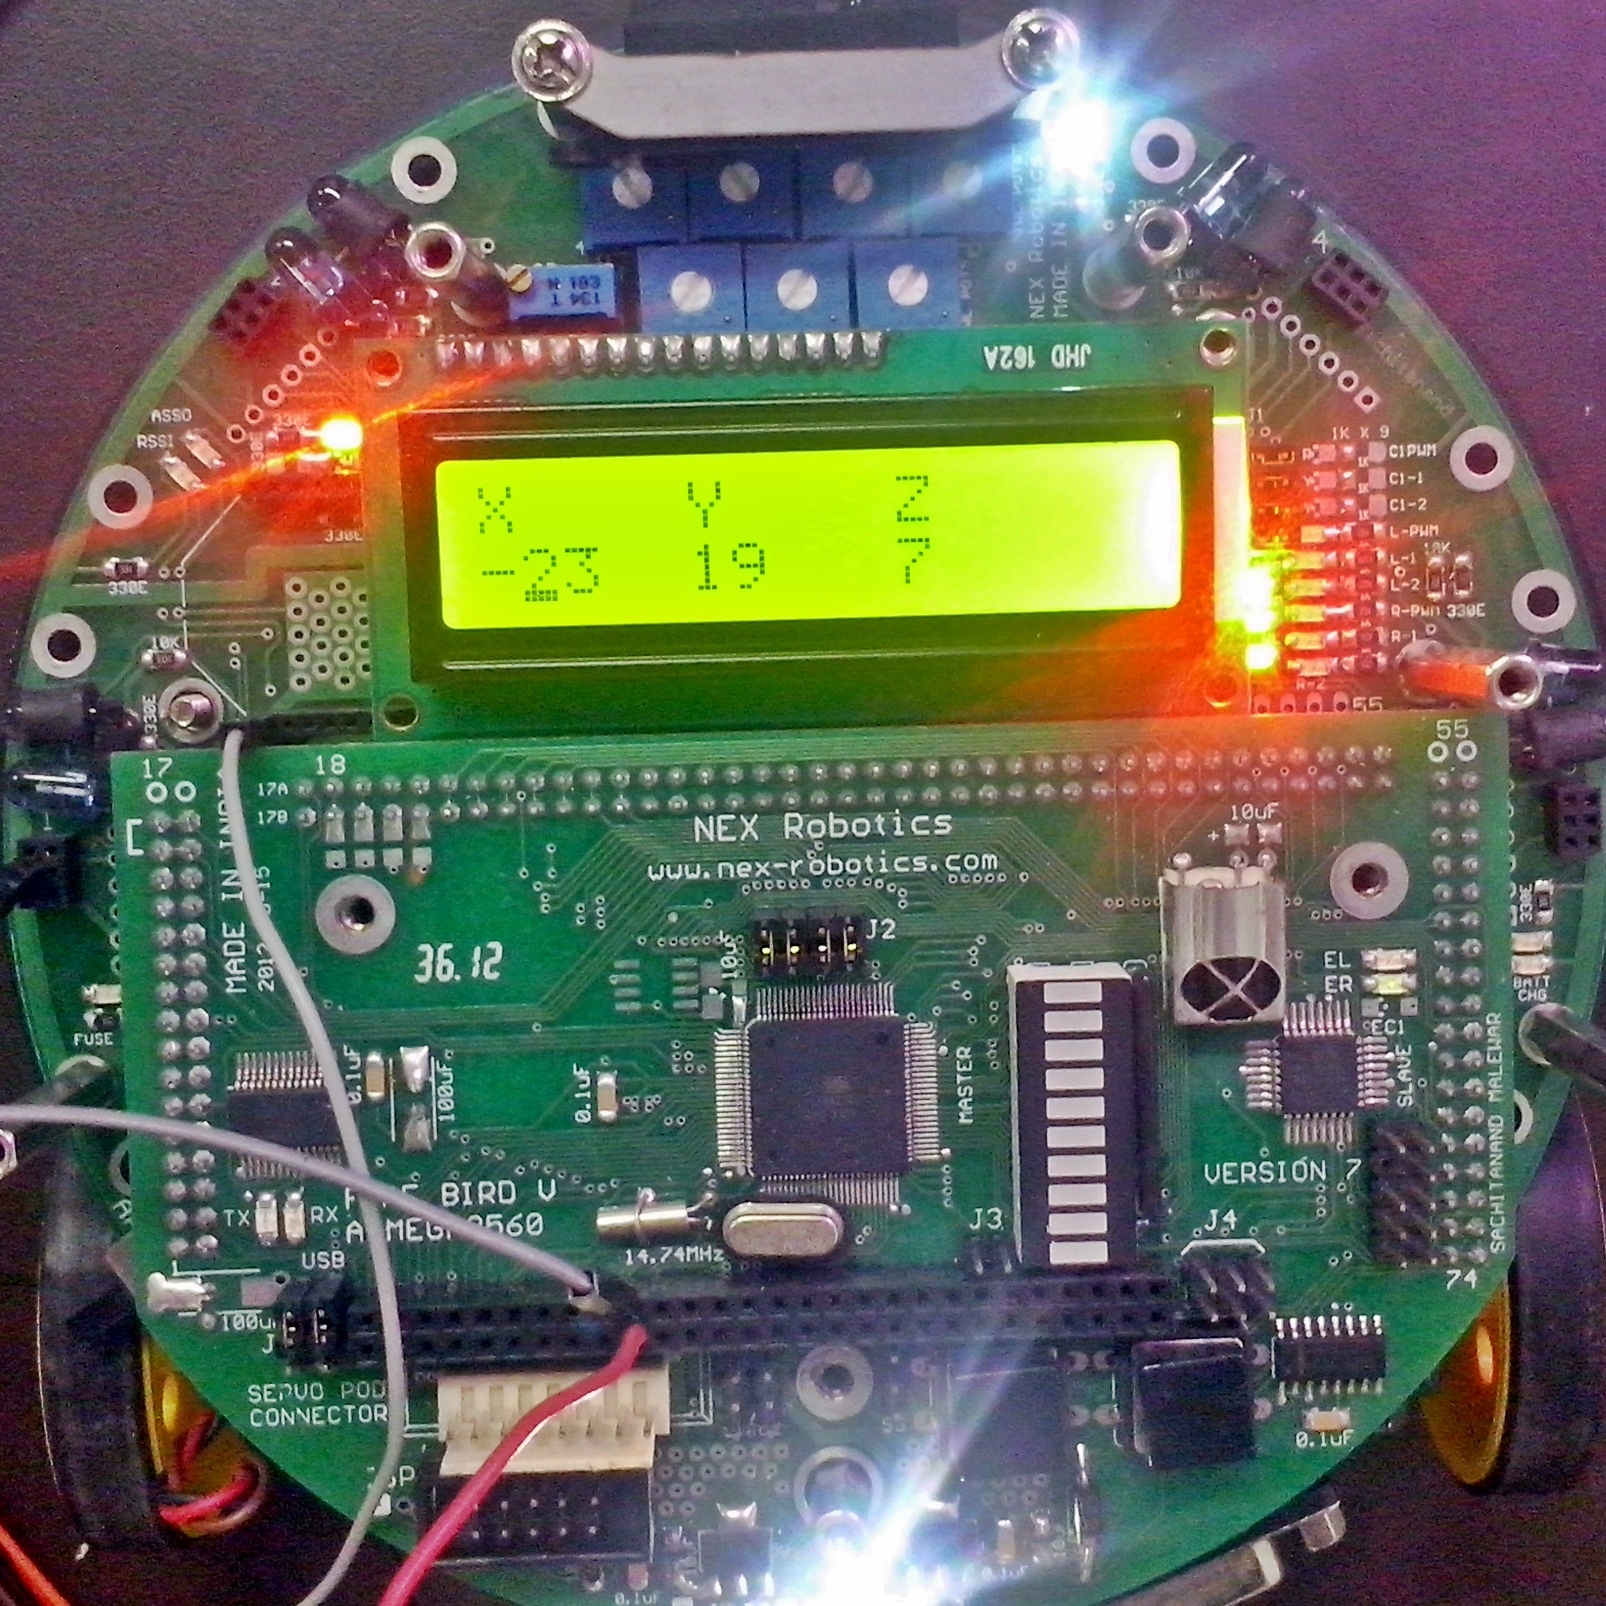
\includegraphics[scale=0.40]{CAM00213.jpg}
\end{center}
\caption{Output of Gyroscope on LCD}
\label{fig:1}
\end{figure}



\section{Applications}
\begin{itemize}
\item Quadrotor
\item Balancing robots
\item  Advance robotics
\item Navigation 
\item Motion Control with MMI (Man Machine Interface)
\item Gaming and virtual reality input devices
\end{itemize}

\begin{figure}[!h]
        \centering
        \begin{subfigure}[b]{0.3\textwidth}
                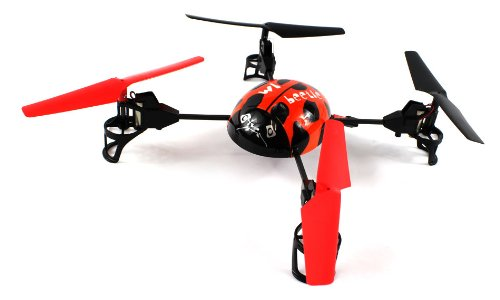
\includegraphics[width=\textwidth]{gyr3.jpg}
                \caption{Quadrotor}
                \label{fig:gull}
        \end{subfigure}%
        ~ %add desired spacing between images, e. g. ~, \quad, \qquad, \hfill etc.
          %(or a blank line to force the subfigure onto a new line)
        \begin{subfigure}[b]{0.3\textwidth}
                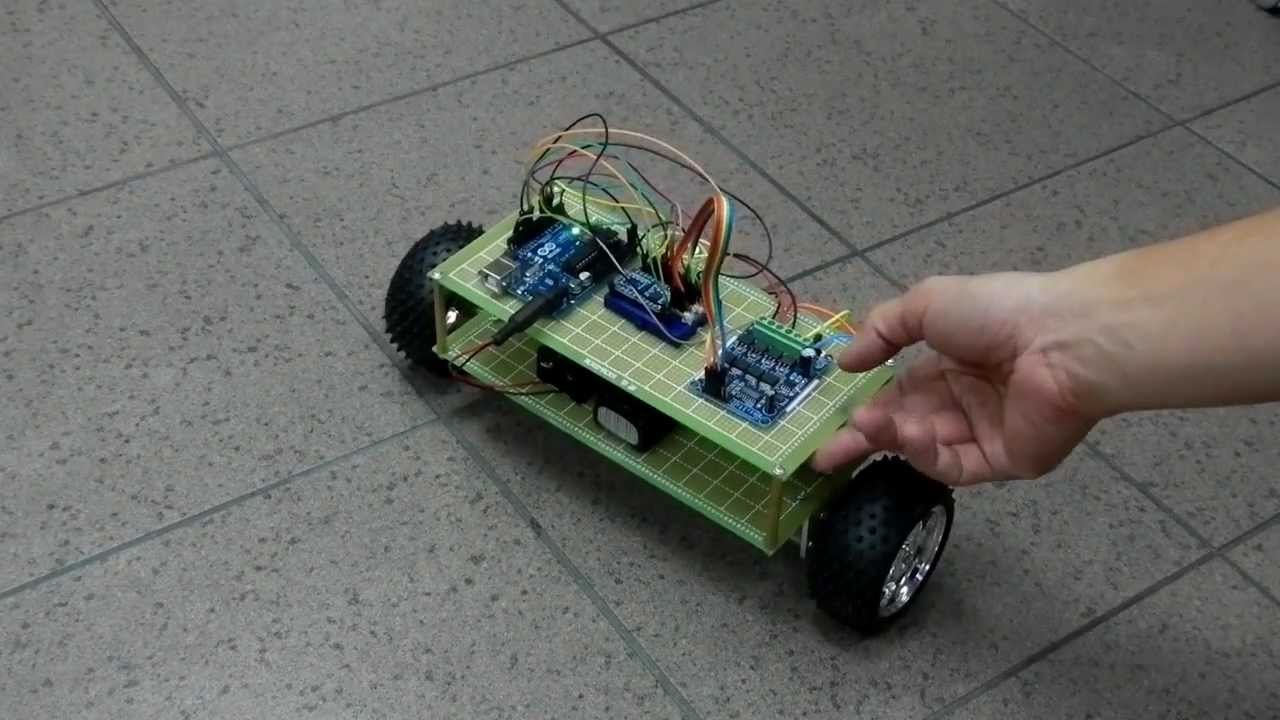
\includegraphics[width=\textwidth]{gyr4.jpg}
                \caption{Self-Balancing Robot}
                \label{fig:tiger}
        \end{subfigure}
        ~ %add desired spacing between images, e. g. ~, \quad, \qquad, \hfill etc.
          %(or a blank line to force the subfigure onto a new line)
        \begin{subfigure}[b]{0.3\textwidth}
                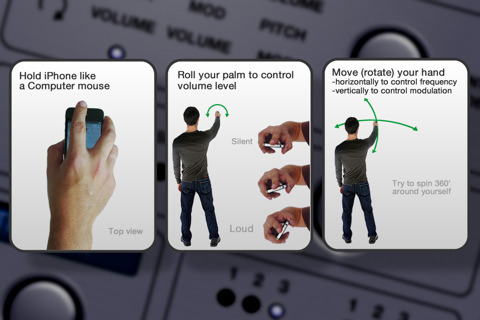
\includegraphics[width=\textwidth]{gyr6.jpg}
                \caption{Gyroscope in Gaming}
                \label{fig:mouse}
        \end{subfigure}
        \caption{Gyroscope Applications}\label{fig:animal}
\end{figure}

\newpage
\section{Reference}
\begin{enumerate}
\item L3G4200D IMU datasheet.
\item LSM303DLHC accelerometer datasheet.
\item ATMEGA 2560 datasheet.
\end{enumerate}
\end{document}